\documentclass[11pt]{article}
\usepackage[utf8]{inputenc}
\usepackage[T1]{fontenc}
\usepackage{amsmath,amssymb,amsfonts}
\usepackage{tgtermes}
\usepackage{newtxmath}
\usepackage[version=4]{mhchem}
\usepackage{graphicx}
\usepackage{booktabs}
\usepackage{siunitx}
\usepackage[margin=1in]{geometry}
\emergencystretch=2em
\usepackage[hidelinks]{hyperref}
\usepackage[numbers,sort&compress]{natbib}
\usepackage{xcolor}
\usepackage{authblk}
\usepackage{caption}
\usepackage{float}
\captionsetup{font=small,labelfont=bf}
\sisetup{detect-all}
\DeclareSIUnit{\Molar}{M}
\graphicspath{{figures_R582/}}

\title{\bfseries A positive-electrode model separating iodine saturation from accessibility loss in zinc--iodine flow batteries}

\author{\textit{[Verified author list and order required]}}
\affil{\textit{[Verified affiliations and corresponding-author details required]}}
\date{}

\begin{document}
\maketitle

\begin{abstract}
During high-capacity charging of zinc-iodine flow batteries, the porous positive electrode must accommodate dissolved and solid iodine while preserving electrochemically accessible area. Full-cell voltage combines these states and cannot resolve them independently. We developed a state-resolved positive-electrode model that separates free-$\ce{I2}$ supersaturation, solid-$\ce{I2}$ inventory and calibrated accessibility loss. Existing full-cell records show a late-charge voltage feature and changing coulombic efficiency across a recorded same-cell current sequence, anchoring the device-scale problem. At $40~\mathrm{mA~cm^{-2}}$, the baseline simulation reaches average saturation at $83.0~\mathrm{mAh~cm^{-2}}$ and 50\% calibrated accessibility loss at $99.6~\mathrm{mAh~cm^{-2}}$. Replacing only the accessibility relation shifts the saturation marker by $0.002~\mathrm{mAh~cm^{-2}}$, prevents 50\% accessibility loss within $120~\mathrm{mAh~cm^{-2}}$ in the matched variant and lowers its terminal voltage by 288 mV. The pore network retains 98--99\% relative permeability at the simulated solid loading, while applied current and oxidized-iodine diffusivity produce large, directionally interpretable shifts in saturation capacity over the selected simulated ranges. The results separate upstream iodine saturation from downstream accessibility feedback and show why voltage alone cannot identify the inventory-to-accessibility relation.
\end{abstract}

\noindent\textbf{Keywords:} zinc-iodine flow battery; porous positive electrode; iodine supersaturation; solid iodine; accessible area; continuum modeling; mass transport

\section{Introduction}


High areal loading in zinc-iodine flow batteries (ZIFBs) places the porous positive electrode under a coupled chemical and transport burden. During charge, iodide is oxidized inside a carbon felt that must accommodate an increasing oxidized-iodine inventory without losing its connected reaction area. This requirement becomes more demanding as current density and charge passed increase. The distinction is especially important at high areal capacity, where iodine inventory can grow well before a terminal voltage excursion. Over the past decade, zinc--polyiodide flow batteries have combined high-energy iodide chemistry with electrolyte, membrane and cell-design strategies for improved power and cycling performance \citep{Li2015,Xie2018,Weng2017,Fan2024}. Yet a full-cell voltage profile does not reveal which positive-electrode state limits the late charge response. Dissolved iodine, retained solid iodine and the remaining reactive surface can change on different spatial and capacity scales, although they are often represented by a single empirical loss term.

Iodine speciation makes this distinction important. The positive reaction produces molecular iodine, $2\ce{I^- -> I2 + 2e^-}$. In excess iodide, aqueous $\ce{I2}$ is partitioned by the $\ce{I2 + I^- <=> I3^-}$ equilibrium; $\ce{I3^-}$ is commonly treated as the dominant soluble polyiodide \citep{Palmer1984,Wen2025}. The total oxidized-iodine inventory can rise while the free $\ce{I2}$ concentration remains buffered below saturation. Once local free $\ce{I2}$ exceeds its effective solubility, solid $\ce{I2}$ can be retained in the felt. Retention alone, however, does not define electrode deactivation. Confined carbon hosts can store substantial solid iodine while maintaining electrochemical reversibility \citep{SolidI2_NatCommun2020,Fitzek2023}, whereas a dense iodine film has been associated with a large increase in positive-electrode charge-transfer resistance under other conditions \citep{Jang2021}. Optical observations in a different iodine cell also show that deposited iodine can change from a continuous charged-state feature to separated residual particles after discharge \citep{LiDualPlate2025}. These studies establish that host geometry and iodine placement matter, but their morphologies and numerical thresholds cannot be transferred directly to the present carbon felt.

The unresolved quantity is the relation between retained solid inventory and electrochemically accessible area. Porous-electrode theory resolves coupled current and species transport \citep{Newman1962,Tichter2020}; flow-battery extensions calculate concentration, current and potential distributions across porous cells \citep{Chakrabarti2020,AparicioMauricio2023}. Studies of other solid-product electrodes, including reduced-order modeling and operando characterization, show how precipitation can alter reaction area and transport \citep{LiS_ROM_JES2025,ZnO_EEM2024,Li2S_EcoMat2024}. For the ZIFB positive electrode, however, neither the onset of average free-$\ce{I2}$ saturation nor a full-cell voltage curve uniquely specifies the accessibility loss caused by retained iodine. An electrode-resolved model must represent three states separately: free-$\ce{I2}$ supersaturation, solid-$\ce{I2}$ inventory and remaining accessible area. It must also distinguish smooth bulk permeability loss from local accessibility feedback, because the two channels need not evolve together.

Here we combine existing full-cell records with a two-dimensional positive-electrode model and independent molecular and mesoscale calculations. The full-cell data establish the late-charge feature and variation across a recorded same-cell current sequence that motivate the analysis. The continuum model then resolves free-$\ce{I2}$ supersaturation, retained solid and accessible area across the porous positive electrode. Periodic density-functional theory (DFT) constrains relative iodine placement on carbon sites, molecular dynamics (MD) bounds oxidized-iodine mobility, a single-fiber calculation defines geometric accessibility families and a pore network quantifies smooth permeability loss. At $40~\mathrm{mA~cm^{-2}}$, the baseline simulation places average saturation at $83.0~\mathrm{mAh~cm^{-2}}$ and 50\% calibrated accessibility loss at $99.6~\mathrm{mAh~cm^{-2}}$. A matched model containing a different accessibility relation retains nearly the same saturation point but develops a markedly different solid inventory and terminal voltage. This controlled comparison identifies the inventory-to-accessibility relation as the main unresolved link between iodine accumulation and the modeled late-charge response.

\section{Methods summary}


\subsection{Existing full-cell records}


The experimental analysis uses previously acquired ZIFB full-cell records. They include a representative charge profile at $40~\mathrm{mA~cm^{-2}}$ and a same-cell pristine rate sequence from 80 to $360~\mathrm{mA~cm^{-2}}$. Separate records at 40 and $400~\mathrm{mA~cm^{-2}}$ complement four consecutive cycles used to evaluate the late-charge voltage feature. Each physical file or cell remains the independent unit. Sequential cycles are shown as within-cell ranges and are not treated as independent replicates. The separate 40 mA cm$^{-2}$ pristine cell remains visually and statistically distinct from the pristine 80--360 mA cm$^{-2}$ sequence. The 400 mA cm$^{-2}$ cell with a P350C positive electrode is also kept separate.

The representative voltage profile was interpolated on a $0.25~\mathrm{mAh~cm^{-2}}$ grid. A cubic Savitzky--Golay derivative \citep{Savitzky1964} with a primary window of $10.25~\mathrm{mAh~cm^{-2}}$ was used to locate the rise onset and the maximum of $\mathrm{d}V/\mathrm{d}Q$. Windows of 5.25 and $15.25~\mathrm{mAh~cm^{-2}}$ provided estimator-sensitivity ranges. These ranges describe the effect of a prespecified processing choice and are not confidence intervals. The derivative landmarks were not used to set $Q_s$ or $Q_{f,\mathrm{cal}}$; these coordinates were read from the pre-existing calibrated continuum branch. The same full-cell record is used separately in the reduced observation-layer fit (Supplementary Fig.~S6), so the overlay is not independent validation.

All legacy acquisition filenames or condition fields containing \texttt{NH4Cl}, including capitalization variants, refer to experiments performed with $\ce{NH4Br}$; the discrepancy is the metadata-entry error EXP-META-001. Raw filenames, file contents and hashes are preserved, while processed tables use the corrected identity.

\subsection{Positive-electrode continuum model}


The continuum model represents a $4~\mathrm{cm^2}$ flow cell with a 2 mm porous carbon-felt positive electrode, a Nafion 212 separator, a 25 mL reservoir and $50~\mathrm{mL~min^{-1}}$ recirculation. The baseline electrolyte is $1~\mathrm{M}~\ce{ZnI2}+4~\mathrm{M}~\ce{NH4Br}$ at 293.15 K; this salt mixture serves as a representative supporting electrolyte. Bromide contributes to the prescribed iodine complexation relation and supporting-electrolyte properties; the modeled faradaic couple is $\ce{I2/I^-}$. The baseline charge uses $40~\mathrm{mA~cm^{-2}}$.

The two-dimensional positive-electrode domain spans $x=3$-5 mm from the current collector to the separator and $y=0$-20 mm along electrolyte flow. COMSOL Multiphysics 6.3.0.290, COMSOL AB, Stockholm, Sweden, was used to solve a Tertiary Current Distribution, Nernst--Planck model coupled to Free and Porous Media Flow with the porous-domain Darcian setting and advective--diffusive transport. The dissolved oxidized species were treated as a locally equilibrated lumped pool, $c_O$. The selected $\ce{I2}/\ce{I^-}/\ce{I3^-}$ coefficient is near the value reported by Palmer et al. \citep{Palmer1984}. The conditional bromide-complexation coefficient is a rounded prior near Lee et al.'s value, while Park et al. and Weng et al. provide system-specific precedent for $\ce{I2Br^-}$ formation \citep{Lee2023,Park2021,Weng2017}. The remaining iodide concentration is reconstructed from the oxidized inventory through a stoichiometric algebraic relation. This reduction avoids assigning independent transport equations to species that the present data cannot identify separately.

Under the local-equilibrium reduction, the dissolved oxidized pool is partitioned into free $\ce{I2}$ according to

\[
c_{\ce{I2}}^{\mathrm{free}}=\frac{c_O}{\beta}, \qquad
\beta=1+K_{\mathrm I}c_{\ce{I^-}}+K_{\mathrm{Br}}c_{\ce{Br^-}}.
\]

The local supersaturation ratio is $S=c_{\ce{I2}}^{\mathrm{free}}/c_{\mathrm{sat}}^{\mathrm{eff}}$. Here $c_{\mathrm{sat}}=\SI{1.33}{mol.m^{-3}}$ is the dilute-water intrinsic $\ce{I2}$ solubility reference \citep{Ramette1965}. The baseline uses $c_{\mathrm{sat}}^{\mathrm{eff}}=c_{\mathrm{sat}}/\gamma_{\mathrm{salt}}$ with $\gamma_{\mathrm{salt}}=3$; this factor is a bounded cross-salt prior constrained by ionic-strength and salting behavior \citep{Palmer1984}, with $\gamma_{\mathrm{salt}}=2$--4 used for sensitivity analysis. Thus $c_{\mathrm{sat}}^{\mathrm{eff}}\approx\SI{0.44}{mol.m^{-3}}$ is model-derived rather than a measured apparent solubility for the baseline supporting electrolyte. The positive-electrode average reaches the saturation marker, $Q_s$, when $\langle S\rangle=1$. Local values can exceed unity before this average crossing. A supersaturation-gated deposited-iodine pathway advances the solid-$\ce{I2}$ volume fraction, $\varepsilon_s$, while the soluble-iodine pathway follows Butler-Volmer kinetics. Electronic and ionic currents are conserved across the domain, and the two reaction currents sum to the imposed current.

The baseline accessibility relation maps the solid state and a dynamic iodine-placement variable onto the fractional accessibility loss, $\theta_{\mathrm{cal}}$. We define the calibration-controlled remaining-accessibility factor as $R_\theta=1-\theta_{\mathrm{cal}}$. In the solved model, the native reaction-area multiplier also contains a separate pore-transmissibility factor,

\[
R_\theta=1-\theta_{\mathrm{cal}},\qquad
\frac{A_{\mathrm{bare}}}{A_0}=R_\theta T_{\mathrm{pore}},\qquad
T_{\mathrm{pore}}=\left(\frac{K}{K_0}\right)^{1/2}.
\]

The full product $A_{\mathrm{bare}}/A_0$, not $R_\theta$ alone, multiplies the reactive carbon area. The capacity $Q_{f,\mathrm{cal}}$ is defined by $\langle\theta_{\mathrm{cal}}\rangle=0.5$. Its magnitude is calibrated through the voltage response, making $R_\theta$ an effective electrode-scale relation; $S$ and $\varepsilon_s$ remain separate model states. Solid loading also modifies diffusivity, conductivity and smooth relative permeability through porosity-dependent algebraic relations. Model pressure is hydraulic; the electrical response is calculated from the solid- and liquid-phase potentials.

\subsection{Matched accessibility comparison and numerical checks}


A matched simulation replaced only the baseline accessibility expression with a dense island-model relation,

\[
\theta_{\mathrm{island}}=1-\exp\left(-35.4\,\varepsilon_{s,\mathrm{reg}}^{0.6222}\right).
\]

The baseline and island-model simulations used identical geometry, mesh, time grid, transport properties, kinetic parameters and solver tolerances. Both calculations contained 7776 finite elements and used a relative tolerance of $3\times10^{-4}$. A second, one-way calculation evaluated the island relation on the baseline solid inventory without feeding the resulting area back into the reaction equations. This three-curve comparison separates the direct mapping from the coupled response of current, solid accumulation and voltage. A coarser-mesh comparison and a tighter-tolerance calculation gave the same endpoint voltage difference within the predefined numerical checks. Input identity, software objects and output hashes are retained in the source-data package rather than in the scientific narrative.

\subsection{Molecular calculations}


Periodic DFT calculations used CP2K/Quickstep \citep{Kuhne2020CP2K,VandeVondele2005Quickstep}, the PBE exchange-correlation functional \citep{Perdew1996PBE}, D3(BJ) dispersion \citep{Grimme2010D3,Grimme2011D3BJ}, DZVP-MOLOPT-SR-GTH basis sets \citep{VandeVondele2007MOLOPT} and GTH pseudopotentials \citep{Goedecker1996GTH,Hartwigsen1998GTH,Krack2005GTHPBE}. The electronic-density cutoff was 150 Ry, the relative cutoff was 30 Ry and periodic carbon models were sampled at the $\Gamma$ point. Geometry optimizations compared one $\ce{I2}$ molecule at basal, carbonyl, hydroxyl and vacancy sites. Counterpoise-corrected single-point energies were used for the site ordering \citep{Boys1970Counterpoise}. These values compare electronic energies within a finite computational setup; they are not solution free energies or nucleation barriers.

Classical MD used GROMACS \citep{Abraham2015GROMACS} and SPC/E water \citep{Berendsen1987SPCE} for the baseline electrolyte. Halide parameters followed the Joung-Cheatham family \citep{Joung2008Ions}, while the oxidized-iodine species used project-specific analogue parameterizations. Initial configurations were prepared with Packmol \citep{Martinez2009Packmol}. Each state-of-charge composition was minimized, equilibrated for 0.1 ns in NVT and 0.5 ns in NPT, and propagated for one 20 ns NVT trajectory at 298.15 K. Diffusivities were obtained from center-of-mass mean-squared displacements over a 2.51-8.49 ns lag interval. Four contiguous 5 ns blocks characterize within-trajectory stability. They do not provide an independent-replica standard error. Electronic-continuum charge scaling was compared with formal ionic charges \citep{Leontyev2009ECC}; the resulting range is used as a mobility prior.

\subsection{Single-fiber and pore-network calculations}


The single-fiber model represents a $7.5~\mu\mathrm{m}$ carbon fiber in a cylindrical unit cell with initial liquid fraction 0.85. Deposited volume is distributed among idealized island populations, and a finite-difference diffusion calculation determines the remaining accessible-area fraction. The main comparison uses areal number densities of $10^{11}$ and $10^{14}~\mathrm{m^{-2}}$ to span sparse and dense placement families. These geometries define possible inventory-to-accessibility relations; the DFT calculations do not set the island number density.

The pore model contains a $15^3$ network with lognormally distributed throat radii. A sparse symmetric positive-definite solve calculates relative permeability as solid volume is assigned under six placement rules. The calculation resolves smooth changes in the connected hydraulic network but does not represent a discrete deposit image from the ZIFB felt. The single-fiber and pore-network outputs bound accessibility and smooth permeability, respectively.

\subsection{Operating-variable calculations}


The effect of oxidized-iodine mobility was obtained from seven full continuum simulations with $D_{\mathrm{eff}}/D_0$ between 0.5 and 2.0. Current scans ran 20 and $40~\mathrm{mA~cm^{-2}}$ to $Q=120~\mathrm{mAh~cm^{-2}}$, and 80 and $120~\mathrm{mA~cm^{-2}}$ to $Q=40~\mathrm{mAh~cm^{-2}}$. The $80~\mathrm{mA~cm^{-2}}$ simulation ended before the average reached $S=1$. Only the solved 20--40 mA cm$^{-2}$ interval is connected as an interpolation. Additional full simulations varied recirculation rate from 25 to $100~\mathrm{mL~min^{-1}}$ and changed felt thickness and porosity together. The latter comparison is a linked geometry change, not an isolated thickness coefficient.

Because the fiber-scale diffusion layer is below the continuum mesh, a separate analytical calculation varies its thickness with a Sherwood relation, $Sh\propto Re^mSc^{1/3}$. This postprocess is labeled separately from the full simulations. A smooth-permeability substitution is assessed by its endpoint voltage change and is not converted into a saturation capacity. All deterministic curves are shown without inferential error bars.

\section{Results and discussion}


\subsection{Existing full-cell records define the positive-electrode problem}


The full-cell records first establish the device-scale behavior that the positive-electrode model must organize. At $40~\mathrm{mA~cm^{-2}}$, the representative cycle develops a broad late-charge voltage rise rather than a single abrupt transition (Fig.~\ref{fig:experimental-problem}b). The primary derivative analysis locates the rise onset at $52.0~\mathrm{mAh~cm^{-2}}$ and its maximum at $95.0~\mathrm{mAh~cm^{-2}}$. Varying the smoothing window moves these locations, especially near the end of charge, but preserves a distributed voltage-rise interval. This shape is consistent with a state that develops progressively inside a porous electrode. It does not by itself specify whether the change originates from free-iodine accumulation, solid retention, loss of reaction area or the zinc negative electrode.

\begin{figure}[!t]
\centering
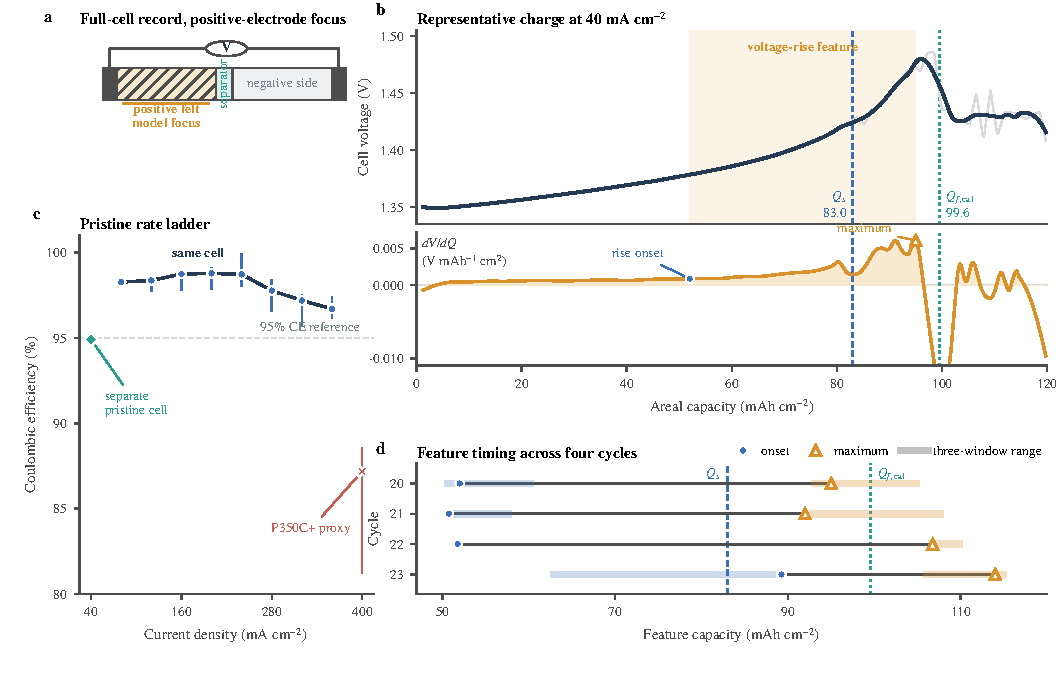
\includegraphics[width=\textwidth]{Fig_R582_experimental_problem.pdf}
\caption{\textbf{Full-cell records motivate a positive-electrode state analysis.}
\textbf{a,} The measured cell response contains both electrodes, whereas the model and interpretation focus on the porous positive carbon felt.
\textbf{b,} Representative cycle-20 charge at 40 mA cm$^{-2}$. The thin grey trace is the registered interpolated voltage, the dark trace is its frozen cubic Savitzky--Golay smooth, and the lower trace is $\mathrm{d}V/\mathrm{d}Q$. The shaded interval contains the voltage-rise feature. $Q_s=83.0$ and $Q_{f,\mathrm{cal}}=99.6$ mAh cm$^{-2}$ are pre-existing calibrated-model coordinates; neither was fitted to the derivative landmarks, and their overlay is not independent validation.
\textbf{c,} Coulombic efficiency for the same-cell pristine 80--360 mA cm$^{-2}$ rate ladder. Symbols are within-cell medians, and vertical bars span the full within-cell minimum--maximum range across available sequential cycles. The separate 40 mA cm$^{-2}$ pristine cell and the 400 mA cm$^{-2}$ P350C-positive/pristine-negative proxy are deliberately unconnected.
\textbf{d,} Primary-window rise onset and maximum for cycles 20--23 from one physical cell. Pale spans give extrema across three prespecified derivative windows and are estimator-sensitivity ranges, not confidence intervals. These records motivate, but do not independently validate, the positive-electrode state model.}
\label{fig:experimental-problem}
\end{figure}

The four-cycle analysis confirms that the voltage feature is not described by one fixed capacity. Primary rise onsets for cycles 20-23 occur at 52.00, 50.75, 51.75 and $89.25~\mathrm{mAh~cm^{-2}}$, whereas the derivative maxima occur at 95.00, 92.00, 106.75 and $114.00~\mathrm{mAh~cm^{-2}}$ (Fig.~\ref{fig:experimental-problem}d). Across the three prespecified windows, 11 of 12 onset values precede the baseline model's $Q_s$, while the maxima fall on both sides of $Q_{f,\mathrm{cal}}$. The full-cell feature supplies a capacity range for comparison, not a one-to-one measurement of either modeled state. The spread also argues against selecting a smoothing-dependent voltage point as a universal positive-electrode threshold.

Rate records provide a second view of the same device-level limitation. In the pristine same-cell sequence, median coulombic efficiency remains near 98-99\% from 80 to $240~\mathrm{mA~cm^{-2}}$ and declines to 96.7\% at $360~\mathrm{mA~cm^{-2}}$ (Fig.~\ref{fig:experimental-problem}c). The separate P350C-positive record gives a median of 87.2\% at $400~\mathrm{mA~cm^{-2}}$, but its different positive electrode and physical cell prevent a continuous extension of the pristine sequence. These data show variation across the recorded current sequence before they identify a rate-specific or electrode-specific cause. Their role is to anchor the need for a state-resolved positive-electrode analysis.

The experimental landmarks and model coordinates are kept as distinct observables in Fig.~\ref{fig:experimental-problem}. The vertical values $Q_s=83.0$ and $Q_{f,\mathrm{cal}}=99.6~\mathrm{mAh~cm^{-2}}$ were calculated before overlay on the representative trace, but $Q_{f,\mathrm{cal}}$ belongs to a voltage-calibrated branch. Their proximity to the broad late-charge interval helps organize the problem but does not independently validate free-$\ce{I2}$ concentration or accessible area. Resolving this ambiguity requires the model to show how its internal states evolve across the same capacity range and which state can alter the voltage response.

\subsection{The model separates saturation, retained solid and accessible area}


The positive-electrode model resolves the chemical and functional states that are combined in the full-cell voltage. Electrolyte flows along the 20 mm in-plane direction while electronic and ionic current cross the 2 mm carbon felt between the current collector and separator (Fig.~\ref{fig:domain-state}a). The model calculates a lumped oxidized-iodine concentration, solid-$\ce{I2}$ volume fraction, electronic and ionic potentials, fluid velocity and reaction current. The local-equilibrium speciation reduction maps the oxidized pool to the free $\ce{I2}$ concentration used in $S$. The soluble inventory can increase without forcing free $\ce{I2}$ to rise in direct proportion.

Three linked quantities govern the positive-electrode response (Fig.~\ref{fig:domain-state}b). First, local $S>1$ activates the deposited-iodine pathway and increases $\varepsilon_s$. Second, the calibrated accessibility relation maps $\varepsilon_s$ and its placement state onto $R_\theta$, while solid-dependent permeability supplies $T_{\mathrm{pore}}$. Third, their product, $A_{\mathrm{bare}}/A_0=R_\theta T_{\mathrm{pore}}$, changes local reaction current and the calculated voltage. The model thus distinguishes a thermodynamic-transport state, a retained inventory and an electrode-scale functional state. Calibration enters $R_\theta$, not the separately defined pore-transmissibility factor. Voltage remains an output of the coupled charge and reaction equations.

\begin{figure}[!t]
\centering

\includegraphics[width=\textwidth]{Fig_R582_domain_state_v2.pdf}
\caption{\textbf{A state-resolved model of the ZIFB positive electrode.}
\textbf{a,} The two-dimensional carbon-felt domain spans $x=3$--5 mm from the current collector to the separator and $y=0$--20 mm along electrolyte flow.
\textbf{b,} Free-\ce{I2} supersaturation, $S$, gates retained solid, $\varepsilon_s$. The calibrated relation gives $R_\theta=1-\theta_{\mathrm{cal}}$; the native reaction-area multiplier is $A_{\mathrm{bare}}/A_0=R_\theta T_{\mathrm{pore}}$, and $V$ is a model output.
\textbf{c,} The baseline simulation reaches average saturation at $Q_s=83.0$ mAh cm$^{-2}$ and 50\% calibrated accessibility loss at $Q_{f,\mathrm{cal}}=99.6$ mAh cm$^{-2}$. The state annotations do not define local onset or microscopic deposit form.}
\label{fig:domain-state}
\end{figure}

At the baseline condition, the positive-electrode average reaches $S=1$ at $Q_s=83.0202~\mathrm{mAh~cm^{-2}}$ (Fig.~\ref{fig:domain-state}c). The mean calibrated accessibility loss reaches 0.5 at $Q_{f,\mathrm{cal}}=99.5901~\mathrm{mAh~cm^{-2}}$. The $16.57~\mathrm{mAh~cm^{-2}}$ interval between these markers arises because average saturation and accessibility are different model events. Local supersaturation and solid formation can begin before the average crossing, while substantial reaction area remains after $Q_s$. This sequence is the model's principal explanation for a distributed late-charge response.

The supporting electrolyte sets one condition for this sequence but does not define its subject. In the baseline formulation, excess iodide and bromide enter the complexation factor $\beta$, and the prescribed bulk transport properties set the rate at which oxidized iodine is redistributed. The electrochemical state of interest remains the porous ZIFB positive electrode. Moving to another supporting electrolyte would require its own diffusivity, conductivity, viscosity, iodine-speciation and solubility inputs. The formulation is a specified boundary condition, not an electrolyte-comparison result.

The model markers also have different physical sensitivity. $Q_s$ is controlled upstream by oxidized-iodine generation, complexation and transport. $Q_{f,\mathrm{cal}}$ is additionally controlled by the selected accessibility relation and its feedback on current. This distinction predicts that changing only the accessibility relation should leave the initial saturation event nearly fixed while altering the later solid and voltage response. Figs.~\ref{fig:spatial-progression} and \ref{fig:closure-identifiability} test that prediction in space and through a matched model comparison.

\subsection{Spatial progression localizes the modeled late-charge response}


Two-dimensional snapshots show how the separated states develop inside the positive electrode. Fig.~\ref{fig:spatial-progression} compares $Q=80$, 100 and $120~\mathrm{mAh~cm^{-2}}$, using the same domain and one fixed scale for each variable. The first snapshot lies just before the average saturation marker, the second lies near $Q_{f,\mathrm{cal}}$ and the third represents late charge. This arrangement allows a direct comparison of where retained solid, remaining area and total reaction current change as charge proceeds.

\begin{figure}[!t]
\centering
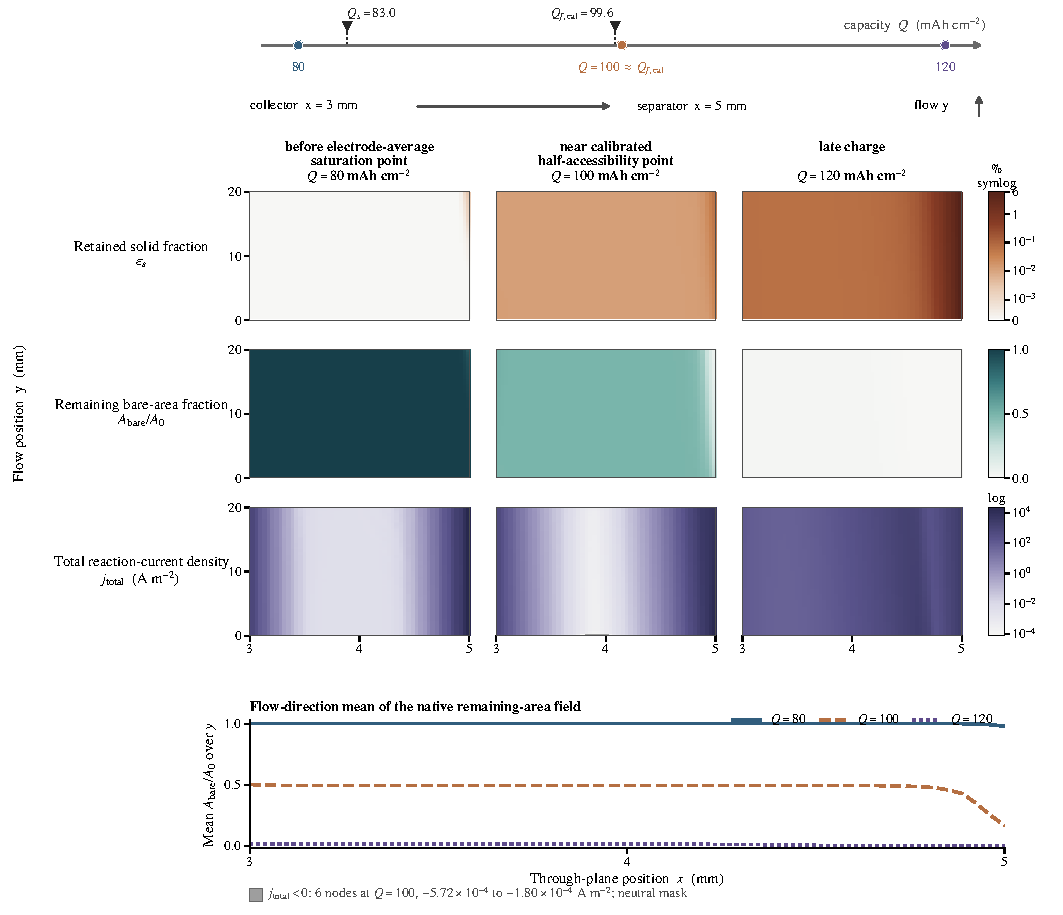
\includegraphics[width=\textwidth]{Fig_R582_spatial_progression_v3.pdf}
\caption{\textbf{Retained solid and native remaining area redistribute reaction within the positive electrode.}
Continuum-model snapshots are shown at $Q=80$, 100 and 120 mAh cm$^{-2}$, respectively before the electrode-average saturation point, near the calibrated half-accessibility point and at late charge. The capacity rail distinguishes the exported snapshots from $Q_s=83.0202$ and $Q_{f,\mathrm{cal}}=99.5901$ mAh cm$^{-2}$; $Q=100$ mAh cm$^{-2}$ is close to, but not identical to, $Q_{f,\mathrm{cal}}$. The map rows show retained-solid fraction, $\varepsilon_s$, native remaining bare-area fraction, $A_{\mathrm{bare}}/A_0$, and total reaction-current density, $j_{\mathrm{total}}$, using one scale per quantity across all capacities. The lower plot gives the arithmetic mean of the native remaining-area field over the uniformly sampled flow coordinate $y$. Six negative-current nodes at $Q=100$ mAh cm$^{-2}$, spanning $-5.72\times10^{-4}$ to $-1.80\times10^{-4}$ A m$^{-2}$, are retained as a neutral mask rather than clipped or converted to magnitudes. Every map uses the same 3--5 mm through-plane and 0--20 mm flow domain. These are continuum-model fields, not micrographs or evidence for a unique deposit morphology or pore-blocking front.}
\label{fig:spatial-progression}
\end{figure}

At $80~\mathrm{mAh~cm^{-2}}$, the electrode average remains below $S=1$, yet the retained-solid field is already spatially nonuniform (Fig.~\ref{fig:spatial-progression}, top row). The result follows from local activation of the deposited-iodine pathway before the mean crossing. By 100 and $120~\mathrm{mAh~cm^{-2}}$, $\varepsilon_s$ increases most strongly toward the separator-facing side. The field is a continuum volume fraction, so its gradient reports where the model retains solid inventory. It carries no information about crystal shape, film continuity or individual pore throats.

The native reaction-area maps, exported directly as $A_{\mathrm{bare}}/A_0=R_\theta T_{\mathrm{pore}}$, expose the functional consequence of the retained-solid field (Fig.~\ref{fig:spatial-progression}, middle row). Near $Q_{f,\mathrm{cal}}$, the separator-facing region has lost a substantial fraction of its native reaction-area multiplier while other parts of the felt remain active. At $120~\mathrm{mAh~cm^{-2}}$, the low-area region has expanded across the through-plane direction. The flow-direction mean below the maps confirms the same separator-side decline without introducing a fitted profile. The spatial progression explains why an electrode-average saturation point can precede a strong voltage response: the late response depends on how local retained inventory is converted into available reaction area.

Reaction current redistributes as the accessibility field changes (Fig.~\ref{fig:spatial-progression}, bottom row). The shared logarithmic scale reveals a broad current range without rescaling individual capacities. Current remains distributed at 80 mAh cm$^{-2}$, becomes more heterogeneous near 100 mAh cm$^{-2}$ and reorganizes further by the endpoint. Six negative nodes at 100 mAh cm$^{-2}$ are retained as a neutral mask, preserving the sign information rather than converting the field to an absolute value. The current map follows the solved accessibility feedback; it is not an independent image of deposited iodine.

The spatial ordering gives the model a clear causal sequence. Oxidized-iodine transport and complexation determine where free $\ce{I2}$ approaches saturation. Local supersaturation then advances the retained-solid state. The accessibility relation converts that inventory into a loss of available carbon area, which redistributes reaction current. Each step corresponds to a modeled quantity. The next question is whether this sequence, especially its late part, is robust to a different inventory-to-area relation.

\subsection{Accessibility feedback controls the late solid and voltage response}


Changing only the accessibility relation has almost no effect on average saturation but strongly changes the later response. In the matched simulations, $Q_s$ is $82.8903~\mathrm{mAh~cm^{-2}}$ for the calibrated baseline and $82.8924~\mathrm{mAh~cm^{-2}}$ for the coupled island-model variant (Fig.~\ref{fig:closure-identifiability}a). The difference is $0.0021~\mathrm{mAh~cm^{-2}}$. This result shows that the initial average saturation event is governed mainly by the common transport and speciation state, before accessibility feedback becomes large.

\begin{figure}[!t]
\centering

\includegraphics[width=\textwidth]{Fig_R582_closure_identifiability.pdf}
\caption{\textbf{Accessibility relation controls the late charge response.}
\textbf{a,} Calibration-controlled remaining-accessibility factor, $R_\theta=1-\theta$, for the calibrated baseline, a one-way island-model shadow evaluated on the baseline solid inventory, and the fully coupled island-model variant. The matched simulations give $Q_s=82.890$ and $82.892$ mAh cm$^{-2}$.
\textbf{b,} Voltage trajectories and the island-minus-baseline difference, which reaches $-288.2$ mV at 120 mAh cm$^{-2}$.
\textbf{c,} Each solved branch's solid-\ce{I2} fraction; horizontal lines mark the solid-fraction values at $R_\theta=0.5$ for the baseline and island relation.
\textbf{d,} Accessibility--coefficient pairs that reproduce the same selected voltage contribution. This controlled model-form sensitivity does not identify deposit morphology.}
\label{fig:closure-identifiability}
\end{figure}

The calibration-controlled remaining accessibility, $R_\theta$, diverges after saturation. The calibrated baseline reaches $\langle\theta_{\mathrm{cal}}\rangle=0.5$ near $99.46~\mathrm{mAh~cm^{-2}}$ and ends with a mean accessibility loss of 0.990. The coupled island-model variant does not reach 50\% loss by $120~\mathrm{mAh~cm^{-2}}$ and ends at 0.309 loss. A one-way island-model shadow evaluated on the baseline solid inventory ends at a much larger loss than the coupled island case. This difference shows why an accessibility curve cannot be applied after the simulation without changing the interpretation. Once $R_\theta$ feeds back through $A_{\mathrm{bare}}/A_0$, it also changes how much solid accumulates.

The coupled voltage curves expose the system-level consequence (Fig.~\ref{fig:closure-identifiability}b). At $120~\mathrm{mAh~cm^{-2}}$, the calibrated baseline reaches 1.7284 V, whereas the island-model variant reaches 1.4402 V. The island-minus-baseline difference is $-288.2$ mV. All other model inputs are identical, so the separation is attributed to the chosen inventory-to-accessibility relation and its feedback through the reaction equations. The comparison quantifies controlled model-form sensitivity. It does not select one geometric deposit description as the state of the experimental felt.

Each accessibility relation also produces its own solid inventory (Fig.~\ref{fig:closure-identifiability}c). The baseline ends at $\langle\varepsilon_s\rangle=3.152\times10^{-3}$, while the coupled island-model simulation ends at $6.586\times10^{-4}$. The 4.8-fold difference is not imposed directly. It emerges because the remaining-area relation changes the partition and spatial distribution of reaction current, which then changes the deposited-iodine pathway. Solid inventory and accessibility are not equivalent measures of positive-electrode state.

Voltage is also insufficient to recover accessibility uniquely. The degeneracy curve in Fig.~\ref{fig:closure-identifiability}d contains multiple pairs of accessibility loss and voltage coefficient that reproduce the same selected voltage contribution. A voltage fit can trade a larger area loss against a different observation-layer coefficient. Independent information on retained iodine or accessible area is required to distinguish these alternatives. The baseline model thus provides one internally consistent effective relation, not a measurement of deposit morphology.

\subsection{Molecular and mesoscale calculations bound transport and accessibility}


The lower-scale calculations constrain inputs that the full-cell voltage cannot determine independently. Periodic DFT compares BSSE-corrected adsorption energies for one $\ce{I2}$ molecule on representative carbon sites (Fig.~\ref{fig:multiscale-bounds}a). Relative to basal carbon, the hydroxyl and carbonyl sites are lower by 0.595 and 0.446 eV, while the vacancy site is higher by 0.084 eV. This adsorption-energy ordering supports heterogeneous placement as an input to the geometric calculations, but it does not determine island density, solution adsorption free energy or a deposition pathway.

\begin{figure}[!t]
\centering

\includegraphics[width=\textwidth]{Fig_R582_multiscale_bounds_v2.pdf}
\caption{\textbf{Independent bounds on positive-electrode model inputs.}
\textbf{a,} Periodic CP2K BSSE-corrected adsorption energies for dry single-\ce{I2} placement, reported relative to basal carbon.
\textbf{b,} Five-SOC bulk-MD means for \ce{I^-}, \ce{I3^-} and \ce{I2Br^-} under $q=0.8$ ECC and formal-charge parameterizations in the representative \SI{1}{M}~\ce{ZnI2}$+$\SI{4}{M}~\ce{NH4Br} supporting electrolyte; error bars report propagated within-trajectory stability. Shading denotes the formal-charge low-end carrier-proxy range ($0.425$--$0.664\times10^{-9}~\si{m^2.s^{-1}}$), and the dashed line marks the continuum baseline $D_{\mathrm{eff}}=0.50\times10^{-9}~\si{m^2.s^{-1}}$.
\textbf{c,} Geometric remaining area $A/A_0$ for sparse ($N=10^{11}~\si{m^{-2}}$) and dense ($N=10^{14}~\si{m^{-2}}$) single-fibre placement; lines connect computed nodes, including the exact zero-solid boundary.
\textbf{d,} Six-law permeability envelope for an idealized pore network over the baseline solid-\ce{I2} range; the inset retains the full computed range. At $\varepsilon_s=3.219\times10^{-3}$, $K/K_0=0.981$--$0.992$. These lower-scale calculations bound transport and accessibility separately. They do not determine the voltage-calibrated inventory-to-accessibility relation or identify deposit morphology or pore closure.}
\label{fig:multiscale-bounds}
\end{figure}

MD supplies a separate carrier-mobility bound (Fig.~\ref{fig:multiscale-bounds}b). In units of $10^{-9}~\mathrm{m^2~s^{-1}}$, the charge-scaled five-state means for $\ce{I^-}$, $\ce{I3^-}$ and $\ce{I2Br^-}$ are $1.222\pm0.030$, $0.752\pm0.067$ and $0.724\pm0.088$. The oxidized carriers are 38--41\% slower than iodide within this force-field set. Formal charges give 0.708, 0.533 and 0.518, while the continuum baseline is 0.50 in the same units. Each composition contains one trajectory, so the intervals describe within-trajectory stability rather than population uncertainty.

Single-fiber calculations translate solid volume into geometric remaining-area families (Fig.~\ref{fig:multiscale-bounds}c). Sparse placement retains $A/A_0=0.890$ at $\varepsilon_s=3.391\times10^{-3}$, whereas dense placement gives 0.544 at $1.356\times10^{-3}$ and 0.293 at $4.069\times10^{-3}$. Placement density strongly changes geometric accessibility over the continuum solid-loading range. The connecting lines only join computed nodes; they are not a fitted accessibility law and are distinct from the native continuum $A_{\mathrm{bare}}/A_0=R_\theta T_{\mathrm{pore}}$ field.

The pore network isolates the smooth hydraulic consequence of the same loading (Fig.~\ref{fig:multiscale-bounds}d). At $\varepsilon_s=3.219\times10^{-3}$, the six placement rules retain $K/K_0=0.981$--0.992, a loss of only 0.8--1.9\%. Consistently, substituting the continuum permeability relation changes endpoint voltage by 1.27 mV. Smooth bulk permeability is a weak channel in the modeled window, although sub-network constrictions remain a separate physical question.

Together, the calculations separate four uncertainties: relative placement tendency, oxidized-iodine mobility, accessibility at fixed inventory and smooth permeability loss. None supplies the voltage-calibrated accessibility relation. They distinguish physically bounded inputs from the relation that remains to be measured.

A felt can retain a small solid volume without losing much smooth permeability, yet respond strongly in voltage if the same inventory reduces electrochemically accessible area. This distinction is consistent with confined iodine remaining reversible in one carbon host while a dense deposit raises interfacial resistance in another \citep{SolidI2_NatCommun2020,Jang2021}; neither host morphology is assigned to the present felt. Hydraulic connectivity and reactive accessibility require different tests. Pressure drop primarily probes the smooth hydraulic relation, whereas electrode-resolved impedance or reaction-area measurements constrain accessibility.

\subsection{Transport and operating variables shift the modeled saturation window}


Among the selected operating and transport variables highlighted in Fig.~\ref{fig:operating-levers}, applied current and oxidized-iodine diffusivity exert clear modeled leverage on average saturation. Reducing current from 40 to $20~\mathrm{mA~cm^{-2}}$ moves $Q_s$ from 83.02 to $106.32~\mathrm{mAh~cm^{-2}}$ (Fig.~\ref{fig:operating-levers}a), whereas the $120~\mathrm{mA~cm^{-2}}$ marker occurs at $8.39~\mathrm{mAh~cm^{-2}}$. The $80~\mathrm{mA~cm^{-2}}$ run ends before the mean crosses unity and supplies only the bound $Q_s>40~\mathrm{mAh~cm^{-2}}$. Higher current generates oxidized iodine faster than it can be redistributed.

The seven full diffusivity simulations show a similarly strong response (Fig.~\ref{fig:operating-levers}b). Increasing $D_{\mathrm{eff}}/D_0$ from 0.5 to 2.0 moves $Q_s$ monotonically from 45.03 to $106.20~\mathrm{mAh~cm^{-2}}$; the 0.8, 1.0 and 1.5 ratios give 73.13, 83.02 and $97.49~\mathrm{mAh~cm^{-2}}$. Mapping the MD-informed interval of 0.8--1.4 through this solved response gives approximately 73.1--95.0 mAh cm$^{-2}$. Oxidized-iodine diffusivity is thus a high-value input for an electrode-resolved test.

\begin{figure}[!t]
\centering
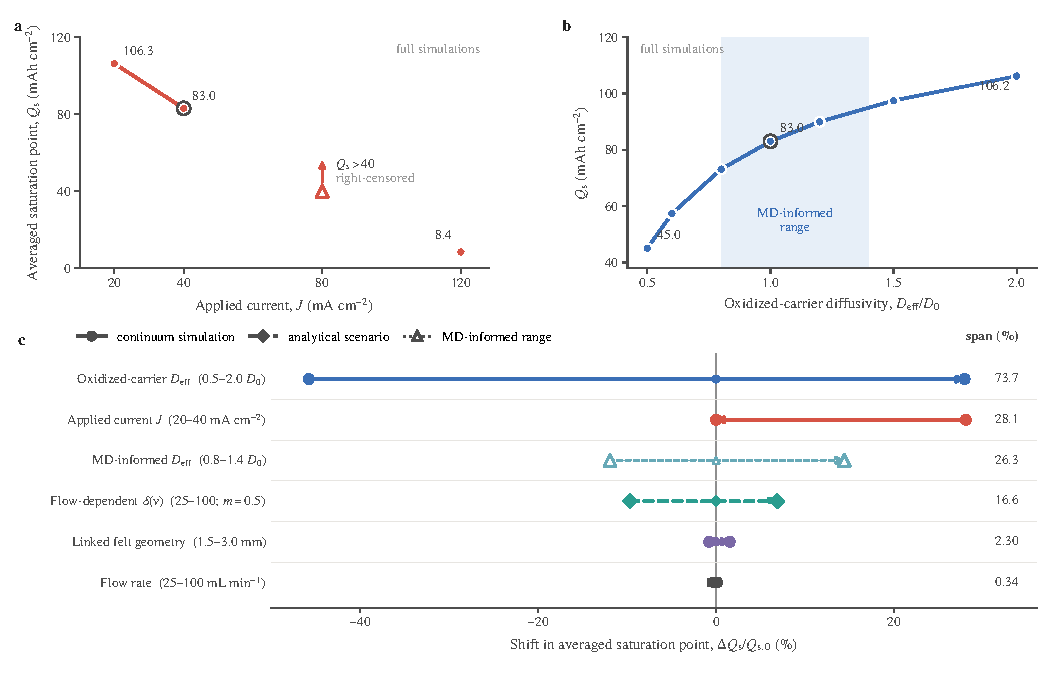
\includegraphics[width=\textwidth]{Fig_R582_operating_levers_v2.pdf}
\caption{\textbf{Applied current and oxidized-carrier diffusivity shift the averaged saturation point.}
\textbf{a,} Positive-electrode-average $S=1$ capacity, $Q_s$, versus applied current. Filled circles denote exact crossings from full continuum simulations. The line connects only the complete 20 and 40 mA cm$^{-2}$ traces. The open triangle at 80 mA cm$^{-2}$ denotes the right-censored result $Q_s>40$ mAh cm$^{-2}$; the separate 120 mA cm$^{-2}$ calculation crosses at 8.39 mAh cm$^{-2}$.
\textbf{b,} $Q_s$ across seven full $D_{\mathrm{eff}}/D_0$ simulations; adjacent points are joined without fitting or extrapolation. Shading marks the MD-informed 0.8--1.4 $D_0$ range.
\textbf{c,} Signed shifts from the baseline $Q_s=83.0202$ mAh cm$^{-2}$. Circles, dashed diamonds and open dotted triangles distinguish full continuum simulations, an analytical boundary-layer scenario and an MD-informed range mapped through the solved diffusivity response. The analytical flow row uses $\delta\propto v^{-0.5}$, and the felt comparison changes thickness and porosity together. The smooth-permeability replacement is reported separately through its $+1.27$ mV endpoint-voltage difference.}
\label{fig:operating-levers}
\end{figure}

Figure~\ref{fig:operating-levers}c places full simulations, an analytical scenario and a bounded prior on one response axis. Full flow simulations at 25, 50 and $100~\mathrm{mL~min^{-1}}$ give $Q_s=82.824$, 83.020 and $83.107~\mathrm{mAh~cm^{-2}}$. Linked changes in felt thickness and porosity span 82.385--84.297 mAh cm$^{-2}$. Both effects are weak because the continuum Darcy field does not resolve the fiber diffusion layer.

An analytical Sherwood scenario tests this sub-grid route. With $m=0.5$, increasing flow from 25 to $100~\mathrm{mL~min^{-1}}$ moves the postprocessed marker from 74.99 to $88.73~\mathrm{mAh~cm^{-2}}$. The 13.74 mAh cm$^{-2}$ span exceeds the full-flow response but remains below the current and diffusivity ranges. Because the boundary-layer relation is changed after the simulation, this is a scenario rather than a solved flow prediction.

The grouped spans also separate upstream from downstream controls. Current and oxidized-carrier diffusivity act on the generation--transport balance and shift $Q_s$. The accessibility relation acts later, changing solid accumulation and voltage with little effect on initial average saturation. Smooth permeability has little voltage leverage at the modeled loading. These responses cannot be represented by one generic transport parameter.

The model prioritizes reducing free-$\ce{I2}$ generation stress and maintaining oxidized-iodine mobility in the positive electrode. Published measurements provide condition-specific current scales and show that solvent environment changes iodine dissolution kinetics \citep{Zhao2022}, although their concentration, method and half-cycle differ from the present charge simulation. The supported design conclusion is directional: lower current and faster oxidized-iodine transport delay modeled saturation, while later voltage depends on deposit accessibility.

The remaining validation need is a pair of independent positive-electrode observables. An iodine-speciation measurement must be combined with retained-iodine or accessible-area information. UV--visible methods quantify dissolved $\ce{I3^-}$ in related systems \citep{ZnNC_AEL2025,WangNatCommun2025PSI}, while impedance can follow iodine-associated interfacial resistance \citep{Jang2021}. Together, such measurements could distinguish the saturation and accessibility states combined in voltage.

The present conclusions apply to a single-charge, porous-positive-electrode model at the stated baseline condition. The model uses a lumped oxidized-iodine carrier, prescribed speciation and mass-transfer relations, and an effective voltage-calibrated accessibility relation. Molecular and mesoscale calculations bound inputs but do not remove this calibration. Negative-electrode morphology, iodine shuttle, discharge redissolution and cycle-to-cycle reset remain full-cell boundary processes. These limits leave the controlled internal comparison intact: average saturation is an upstream transport-speciation event, whereas the later solid inventory and voltage are highly sensitive to accessibility feedback.

\section{Conclusions}


We developed a ZIFB positive-electrode model that separates free-$\ce{I2}$ supersaturation, solid-$\ce{I2}$ inventory and remaining accessible area. Existing full-cell records define the late-charge behavior without assigning it to one electrode state. At $40~\mathrm{mA~cm^{-2}}$, the baseline simulation places average saturation at $83.0~\mathrm{mAh~cm^{-2}}$ and 50\% calibrated accessibility loss at $99.6~\mathrm{mAh~cm^{-2}}$. Replacing only the accessibility relation leaves the saturation point nearly unchanged but alters the later solid inventory and terminal voltage by 288 mV. Molecular and mesoscale calculations identify oxidized-iodine mobility and inventory-to-area mapping as important uncertain inputs, while smooth bulk permeability remains near unity over the simulated loading range. Within the selected operating-variable comparison, current and diffusivity provide directionally clear modeled control of saturation, whereas accessibility controls the downstream voltage response. This testable state sequence still requires an independent measurement of deposit accessibility.

\section*{Data availability}


Processed source data underlying all main and supplementary figures, deterministic analysis and figure-generation code, manuscript sources, and registered model input/output identities are available in the \href{https://github.com/ccyyyYyzz/ZIFB000/tree/r582-zifb-positive-electrode-reproducibility-v1/R582_PUBLICATION_REPRODUCIBILITY}{immutable tagged R582 reproducibility release}. The release includes the continuum-model input hash, study, solution and dataset identities, together with the exact adopted molecular-simulation inputs and output identities. It also includes the operator-confirmed \texttt{EXP-META-001} correction and its preserved raw-file hashes. Raw acquisition files and original solved COMSOL models remain unchanged and are not duplicated in the lightweight repository; their registered identities and SHA-256 hashes are provided for traceability. No repository DOI had been assigned at submission.

\section*{Author contributions}
\emph{[Insert the verified, author-approved CRediT statement before submission.]}

\section*{Acknowledgements}
\emph{[Insert verified funding agencies, grant numbers, sponsor roles and facility acknowledgements before submission.]}

\bibliographystyle{unsrtnat}
\bibliography{refs}

\end{document}
